\newpage
\begin{center}
  \textbf{\large 1. ТЕОРЕТИЧЕСКИЕ И МЕТОДОЛОГИЧЕСКИЕ ОСНОВЫ АВТОМАТИЗАЦИИ ПРЕДПРИЯТИЙ ОБЩЕСТВЕННОГО ПИТАНИЯ}
\end{center}
\refstepcounter{chapter}
\addcontentsline{toc}{chapter}{1. ТЕОРЕТИЧЕСКИЕ И МЕТОДОЛОГИЧЕСКИЕ ОСНОВЫ АВТОМАТИЗАЦИИ ПРЕДПРИЯТИЙ ОБЩЕСТВЕННОГО ПИТАНИЯ}

\section{Цифровизация кафе как многослойная информационная система}

Согласно ГОСТ~34.003-90 \cite{gost34003}, автоматизированная система определяется как система, состоящая из персонала и комплекса средств автоматизации его деятельности, реализующая информационную технологию выполнения установленных функций. Данное определение задает методологически важную рамку: информационная система выходит за пределы отдельного программного продукта и включает пользователей, регламенты, данные, технические средства и процедуры обработки информации. В настоящей работе термин <<автоматизированная информационная система>> (АИС) используется для обозначения такой автоматизированной системы, предметом которой являются сбор, хранение, обработка и передача данных предприятия. Следовательно, кафе целесообразно рассматривать как организационно-техническую систему обслуживания посетителей, в которой кассовые операции, кухня, склад, бронирования, клиентские коммуникации и управленческая аналитика образуют взаимосвязанные информационные потоки.

В прикладной информатике предприятие общественного питания целесообразно рассматривать через несколько функциональных контуров. В операционном контуре фиксируются продажи, заказы, оплаты и возвраты. В производственном контуре заказ связывается с кухней, временем приготовления, статусом выдачи и загрузкой персонала. В учетно-управленческом контуре обрабатываются складские остатки, закупки, себестоимость, финансы и отчетность. В клиентском контуре формируется взаимодействие с гостем: электронное меню, бронирование, профиль, уведомления, обратная связь, программы лояльности и событийные сценарии. Интеграционно-аналитический и защитный контуры обеспечивают обмен данными между модулями, хранение сведений, разграничение доступа и соблюдение правовых требований. Выделение этих контуров опирается на системное понимание автоматизации, при котором программные средства, данные, процедуры и организационные функции рассматриваются во взаимосвязи~\cite{utkin_baldin_2003, kandalenkova2023}.

\begin{table}[H]
\centering
\small
\caption{Основные слои цифровизации предприятия общественного питания}
\label{tab:cafe_digital_layers}
\begin{tabularx}{\textwidth}{|>{\raggedright\arraybackslash}p{0.23\textwidth}|>{\raggedright\arraybackslash}p{0.32\textwidth}|>{\raggedright\arraybackslash}X|}
\hline
\textbf{Слой} & \textbf{Назначение} & \textbf{Типовые компоненты} \\ \hline
Операционный & Фиксация продаж и обслуживание заказа & POS-терминал, касса, платежный модуль, учет чеков \\ \hline
Производственный & Передача заказа в производство и контроль исполнения & Кухонный дисплей, статусы приготовления, маршрут заказа \\ \hline
Учетно-\linebreak управленческий & Контроль ресурсов и экономических показателей & Склад, закупки, финансы, персонал, отчеты \\ \hline
Клиентский & Цифровое взаимодействие с гостем до, во время и после визита & Меню, бронирование, профиль, уведомления, обратная связь \\ \hline
Интеграционно-\linebreak аналитический & Связь модулей и преобразование данных в управленческую информацию & CRM, API, сегментация, аналитические отчеты \\ \hline
Правовой и защитный & Защита информации и выполнение требований законодательства & Роли доступа, согласия, хранение данных, журналирование \\ \hline
\end{tabularx}
\normalsize
\end{table}

Представленная в таблице~\ref{tab:cafe_digital_layers} структура задает аналитическую декомпозицию цифровизации кафе. На практике часть функций малого предприятия может выполняться вручную, часть~--- в рамках одной комплексной платформы, часть~--- через внешние сервисы или заказную разработку. Для проектирования эти слои важно различать, поскольку они предъявляют разные требования к программной системе. Кассовый модуль ориентирован на устойчивую обработку потока заказов, складской модуль~--- на корректный учет остатков и себестоимости, а клиентский контур~--- на понятное, безопасное и удобное взаимодействие гостя с сервисом в условиях ограниченного времени и мобильного доступа.

Архитектурно типовая АИС предприятия питания может быть представлена как совокупность операционного ядра и клиентского контура, соединенных через данные и интеграции. Такая схема сохраняет производственные, учетные и защитные процессы в общей модели и одновременно показывает, что фронтальное взаимодействие с гостем находится на границе между внутренней автоматизацией и воспринимаемым качеством сервиса. Концептуальная структура такой системы представлена на рисунке~\ref{fig:horeca_scheme}.

\begin{figure}[H]
    \centering
    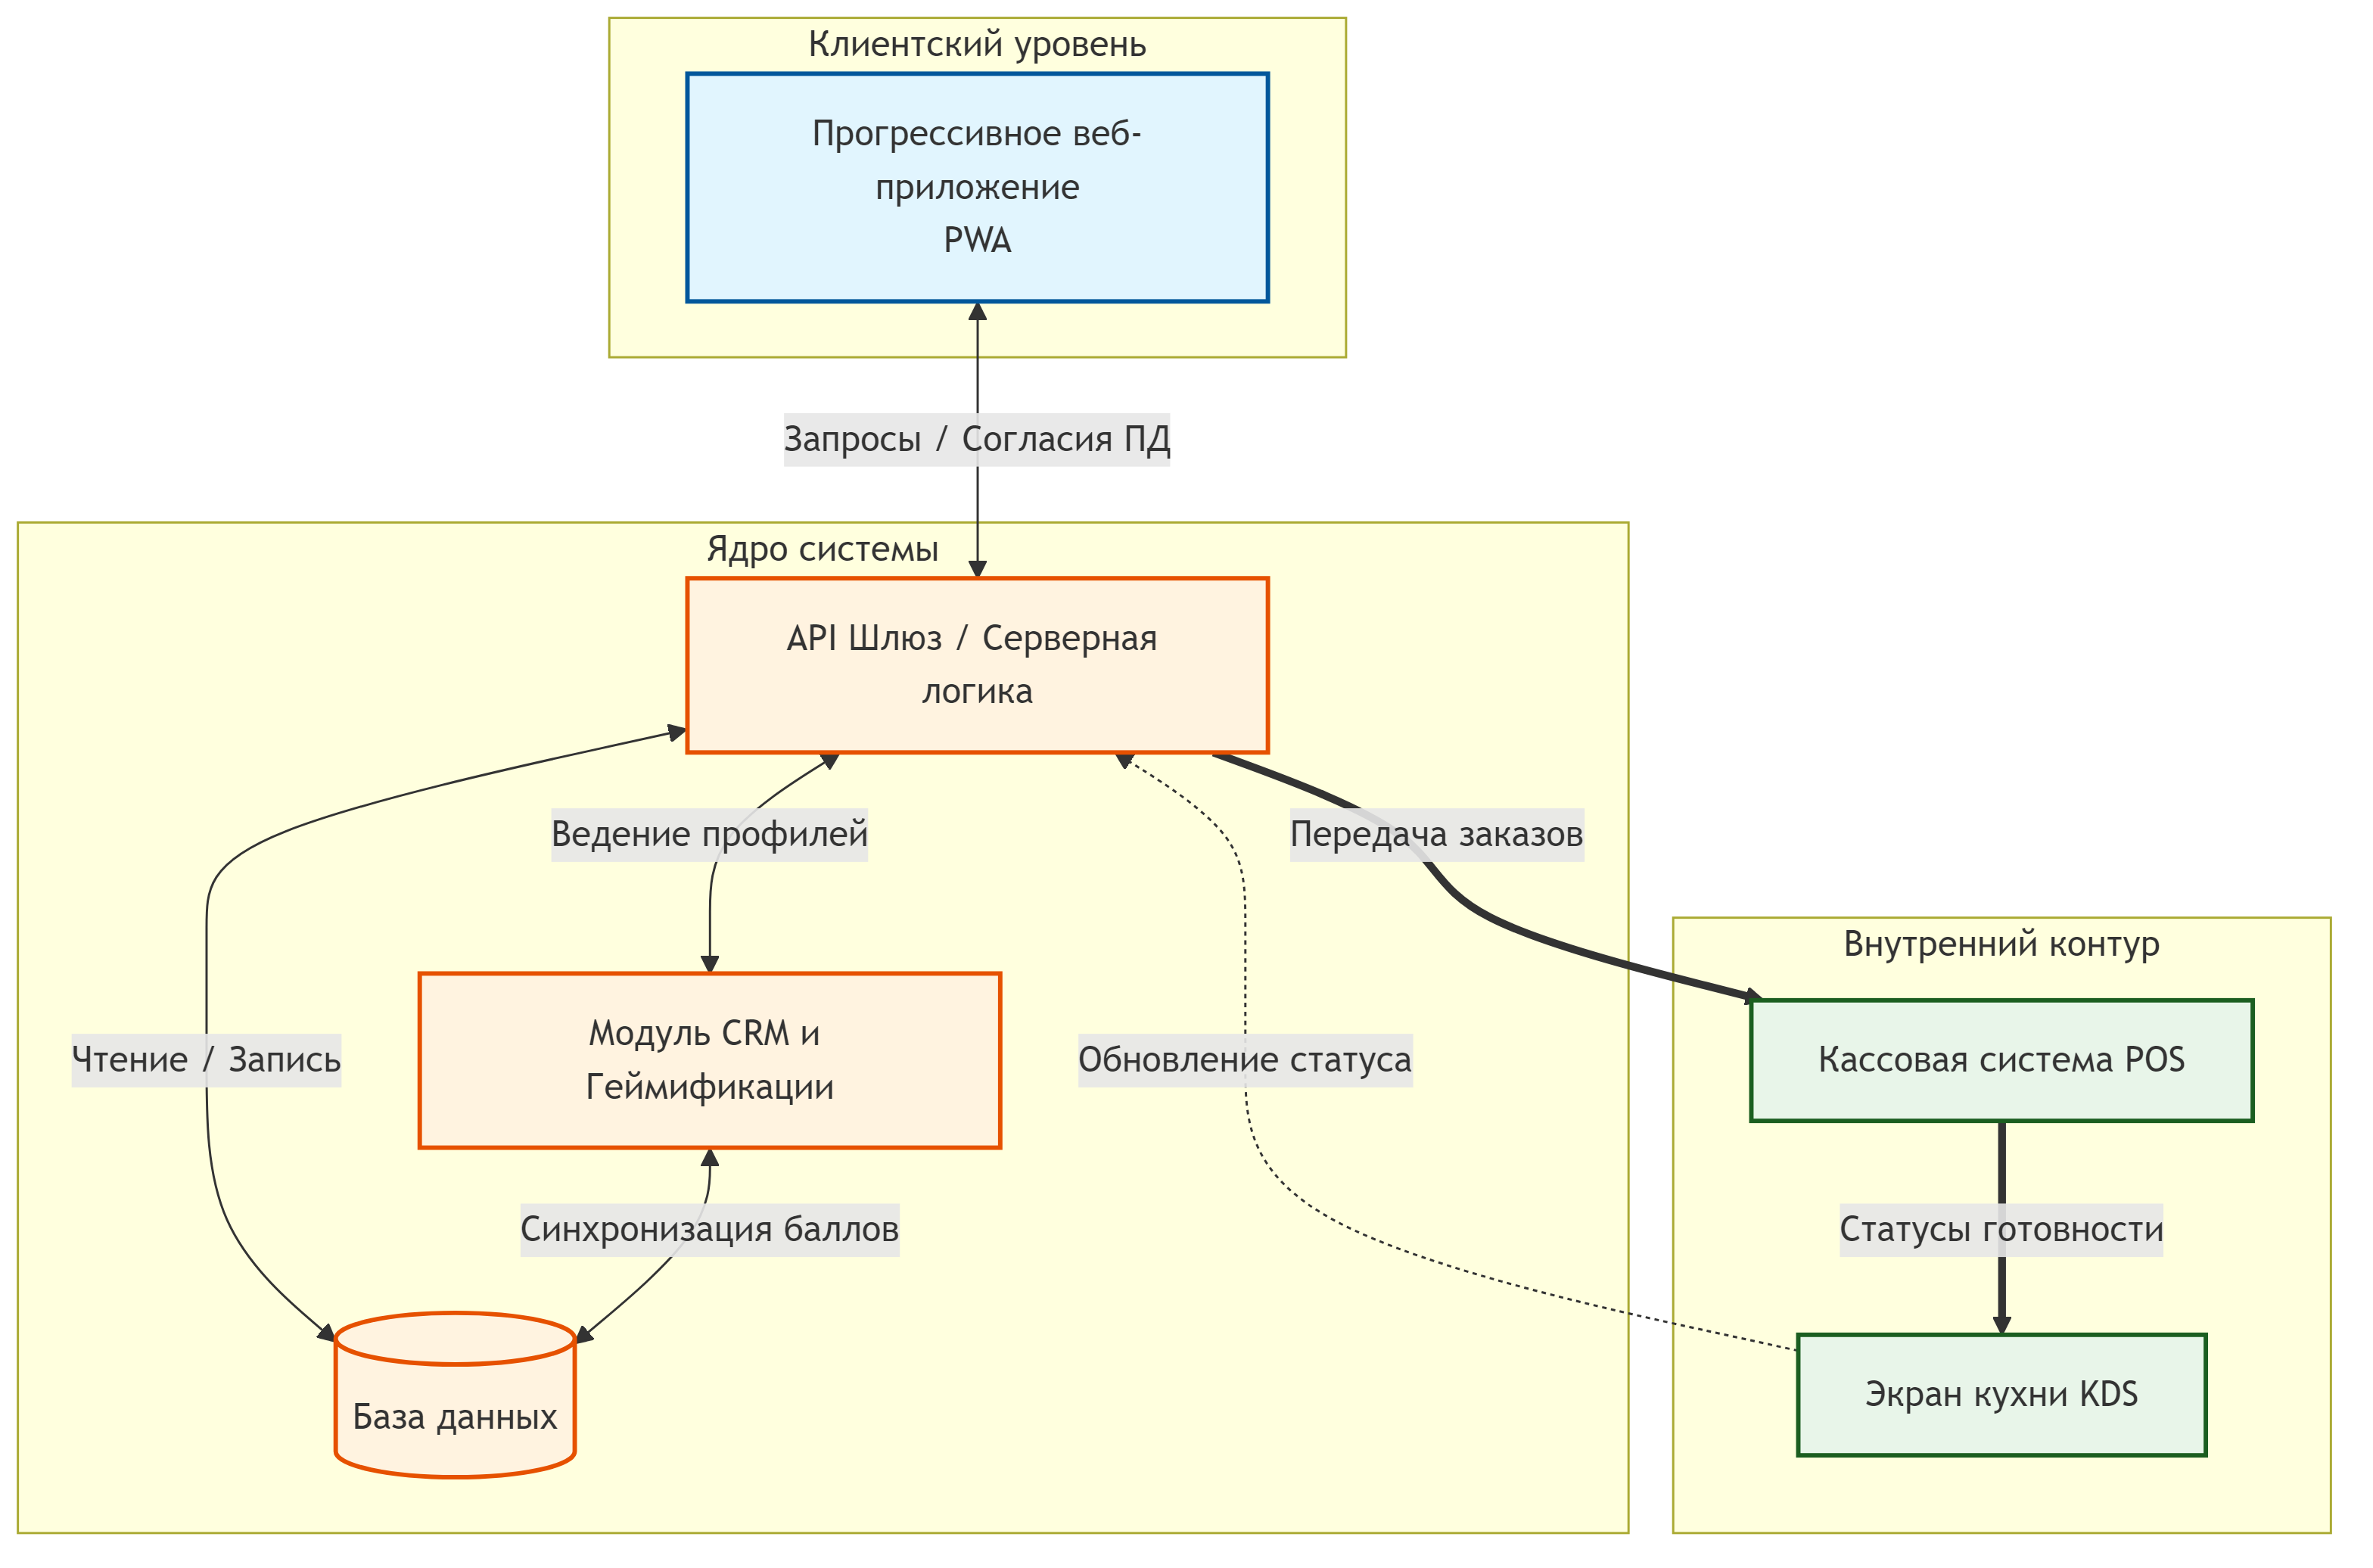
\includegraphics[width=0.85\textwidth]{figures/horeca_architecture_scheme.png}
    \caption{Концептуальная архитектура информационной системы современного кафе}
    \label{fig:horeca_scheme}
\end{figure}

С точки зрения качества программной системы каждый из перечисленных слоев оценивается по функциональным возможностям и нефункциональным характеристикам. Для цифрового сервиса кафе существенны доступность, удобство использования, безопасность, сопровождаемость, интегрируемость и устойчивость к сбоям; эти характеристики входят в современные модели качества программного продукта и архитектурной оценки~\cite{iso25010_2023, bass2021}. В такой постановке наличие электронного меню является лишь частным признаком цифровизации. Более значимым становится вопрос о том, какие слои автоматизации закрываются типовыми решениями, какие остаются зависимыми от ручных процессов и какие требуют специализированного проектирования для конкретного формата заведения.

Таким образом, логика исследования переходит от общей карты цифровизации к классам рыночных решений. Такое сопоставление позволяет выделить клиентский цифровой контур и определить, какие функции взаимодействия с гостем обеспечиваются типовыми средствами, а какие требуют специального проектирования для нового тематического кафе.

\section{Классы рыночных решений для автоматизации предприятий общественного питания}

После выделения функциональных контуров цифровизации необходимо рассмотреть, каким образом они представлены в существующих ИТ-решениях для предприятий общественного питания. Такой обзор выполняет классификационную и проектную функцию: он позволяет соотнести рыночные продукты с отдельными слоями автоматизации и определить, какие задачи могут быть решены типовыми средствами, а какие требуют специализированной разработки с учетом формата рассматриваемого кафе.

Российский рынок ИТ-решений для общественного питания демонстрирует заметную динамику относительно предшествующих периодов. По данным Smart Ranking, суммарная выручка российских ИТ-сервисов для ресторанного сегмента в 2023~году составила 5,8~млрд рублей, увеличившись на 68,3\% по сравнению с предшествующим периодом~\cite{smartranking2024}. В более широком FoodTech-контуре ранее фиксировалась консолидация крупных активов и переход от стратегии быстрого роста к операционной эффективности~\cite{smartranking2022}. Эти сведения фиксируют отраслевой контекст: цифровизация общественного питания оформилась как самостоятельный сегмент ИТ-рынка. Поэтому содержательный анализ требует оценки структуры этого сегмента, то есть определения контуров кафе, которые получают развитую инструментальную поддержку.

Рыночные решения целесообразно группировать по тому, какой слой цифровизации они преимущественно закрывают. Комплексные POS- и ERP-платформы обслуживают операционный, производственный и учетный контуры. Цифровые меню и сервисы заказа создают точечный пользовательский интерфейс для гостя. CRM- и loyalty-решения поддерживают повторные коммуникации и учет клиентской базы. Платформы управления гостевым опытом помогают работать с бронированиями, профилями и персональными предложениями. Наконец, заказные тематические разработки связывают цифровые сценарии с уникальной концепцией бренда, но требуют отдельного проектирования и сопровождения.

К отечественным платформам относятся iiko и R-Keeper. Согласно официальным описаниям, iiko представляет собой облачную ресторанную экосистему, охватывающую продажи, склад, финансы, персонал и доставку~\cite{iiko_official}. R-Keeper развивалась как POS-система для предприятий общественного питания; платформа поддерживает кассовый контур, складской учет, кухонные дисплеи, доставку, CRM и расширения~\cite{rkeeper_official, rkeeper_modules2026}.

Анализ заявленной функциональности комплексных платформ показывает, что их архитектурный центр тяжести находится в операционно-учетном контуре: фиксации продаж, передаче заказа в производство, контроле складских остатков, финансовой отчетности и администрировании процессов обслуживания. Клиентские функции в таких системах присутствуют и чаще встраиваются в логику заказа, доставки, скидок, бонусов или повторных коммуникаций. Тематическое кафе расширяет постановку задачи: цифровой канал сочетает сопровождение транзакции с поддержкой атмосферы заведения, событий, ролевых сценариев и накоплением данных о взаимодействии гостя с концепцией бренда. Поэтому проектирование требует различать операционную автоматизацию предприятия и самостоятельный клиентский слой, ориентированный на управление тематическим опытом.

Локальные клиентские надстройки включают цифровое меню, прием заказа, оплату по QR-коду, уведомления и обратную связь. Например, интеграции наподобие CheckEat расширяют кассовый контур цифровым меню и дистанционным заказом~\cite{poster_checkeat2026}. Их ценность состоит в быстром запуске утилитарного канала обслуживания. По открытым описаниям такие решения преимущественно ориентированы на выбор блюда, оформление заказа и отдельные сервисные действия; длительный сценарий взаимодействия с брендом обычно требует дополнительной проработки.

Зарубежные решения полезны для сравнения при условии учета российского правового и организационного контекста. Платформы Punchh и Paytronix заявляют инструменты лояльности, персональных предложений, мобильных коммуникаций и сценариев повторного обращения~\cite{punchh_loyalty2026, paytronix_mobile2026, paytronix_journey2025}.

SevenRooms, OpenTable и Toast описывают функции управления бронированиями, гостевыми профилями, фирменными мобильными приложениями и коммуникацией с посетителем~\cite{sevenrooms_guestexperience2026, opentable_grm2026, toast_brandedapp2026}. Эти продукты показывают, что клиентский слой может включать более широкий набор функций, чем электронное меню, а их применение в российском тематическом кафе требует адаптации к инфраструктурным, правовым и организационным условиям.

Отдельный интерес представляют заказные тематические разработки. Кейс BAOverse для BAO London иллюстрирует возможность связать посещение разных локаций, фирменную валюту, уровни и эксклюзивные поощрения в единый цифровой сценарий~\cite{baoverse2026}. Значение этого примера состоит в демонстрации принципиально иного уровня клиентского слоя, где цифровая система становится частью тематического опыта. Такие решения имеют брендоспецифичный характер и обычно создаются под конкретную концепцию заведения.

\begin{table}[H]
\centering
\small
\caption{Классы решений и покрываемые ими слои цифровизации кафе}
\label{tab:solution_classes}
\begin{tabularx}{\textwidth}{|>{\raggedright\arraybackslash}p{0.21\textwidth}|>{\raggedright\arraybackslash}p{0.22\textwidth}|>{\raggedright\arraybackslash}p{0.23\textwidth}|>{\raggedright\arraybackslash}X|}
\hline
\textbf{Класс решений} & \textbf{Основной слой} & \textbf{Примеры} & \textbf{Ограничение для тематического кафе} \\ \hline
POS/ERP для ресторанов & Операционный, производственный, учетный & iiko, R-Keeper & Клиентские функции встроены в учет и обслуживание заказа \\ \hline
Цифровое меню и заказ & Клиентский утилитарный интерфейс & QR-меню, CheckEat & Поддерживают отдельные действия гостя и требуют развития для длительного сценария взаимодействия \\ \hline
CRM и loyalty & Повторная коммуникация и клиентская база & Punchh, Paytronix, модули POS & В типовом виде ориентированы на бонусы, предложения и повторные обращения \\ \hline
Guest experience platforms & Бронирования, профили, коммуникации & SevenRooms, OpenTable, Toast & Полезны как ориентир, но требуют адаптации к российскому правовому и организационному контуру \\ \hline
Заказные тематические приложения & Тематический клиентский слой & BAOverse и аналогичные кейсы & Реализуют глубокий сценарий бренда и требуют индивидуального проектирования \\ \hline
\end{tabularx}
\normalsize
\end{table}

Таким образом, в пределах рассмотренной выборки типовые решения наиболее подробно закрывают операционный и учетно-управленческий контуры, тогда как тематически насыщенный клиентский слой чаще требует отдельного проектирования или существенной адаптации. Дальнейший анализ сосредоточен на характеристиках клиентского цифрового контура нового тематического кафе и на данных, которые он способен формировать.

\section{Клиентский цифровой контур и путь гостя}

В настоящей работе клиентский цифровой контур рассматривается как проектное обобщение подходов сервисного дизайна и исследований клиентского взаимодействия в hospitality-среде. Эти подходы связывают качество услуги с последовательностью точек контакта и рассматривают взаимодействие клиента с сервисом на этапах до визита, во время получения услуги и после завершения контакта~\cite{stickdorn2018, chathoth2016}. Поэтому под клиентским цифровым контуром понимается совокупность пользовательских интерфейсов, сервисных сценариев, данных и интеграций, которые сопровождают гостя до визита, во время посещения и после него. Такое определение включает доступ к информации, бронирование, обратную связь, персонализацию, события, уведомления и связь с внутренними процессами кафе.

Для кафе это означает, что цифровой сервис целесообразно проектировать вокруг всей последовательности взаимодействия: от просмотра меню и выбора события до QR-доступа, участия в сценарии внутри заведения, обратной связи, повторного приглашения или персональной рекомендации.

На этапе до визита пользователь может искать информацию о заведении, изучать меню, проверять доступность мероприятий, бронировать столик или оставлять контактные данные. На этапе посещения он взаимодействует с цифровым меню, получает сведения о составе блюд, уточняет правила участия в событии, может фиксировать участие в тематическом сценарии или обращаться к персоналу через цифровой канал. После визита клиентский контур может поддерживать обратную связь, повторные коммуникации, учет предпочтений и приглашения на новые события. Такая логика переводит цифровой сервис из справочного канала в управляемый канал взаимодействия.

\begin{table}[H]
\centering
\small
\caption{Этапы клиентского пути и данные, возникающие в цифровом контуре}
\label{tab:customer_journey_data}
\begin{tabularx}{\textwidth}{|p{0.19\textwidth}|p{0.36\textwidth}|X|}
\hline
\textbf{Этап} & \textbf{Типовые цифровые сценарии} & \textbf{Данные для системы} \\ \hline
До визита & Просмотр меню, изучение событий, бронирование, регистрация интереса & Контакты, дата и цель визита, предпочтения, выбранное событие \\ \hline
Во время визита & QR-меню, уточнение заказа, участие в мероприятии, получение уведомлений & История действий, состав заказа, участие в сценарии, реакции гостя \\ \hline
После визита & Обратная связь, повторное приглашение, персональные предложения & Оценка сервиса, история посещений, интерес к новым событиям \\ \hline
\end{tabularx}
\normalsize
\end{table}

Таблица~\ref{tab:customer_journey_data} показывает две функции клиентского контура: сервисную и информационно-аналитическую. Первая выражается в поддержке действий гостя, вторая~--- в формировании первичных данных о потребностях, поведении и реакции посетителя. Для нового кафе это особенно значимо, поскольку предприятие начинает работу без исторической клиентской базы. В результате проектируемый контур создает основу для будущей CRM-логики уже на ранних этапах взаимодействия с аудиторией.

С позиции HCI/UX клиентский контур предъявляет особые требования к интерфейсу. Пользователь взаимодействует с ним в ситуации реального обслуживания: он может быть ограничен временем, пользоваться смартфоном, находиться в шумном помещении и одновременно общаться с персоналом или другими гостями. Поэтому для такого контура важны понятность навигации, видимость состояния системы, своевременная обратная связь и снижение когнитивной нагрузки~\cite{norman2013}. Ошибки клиентского интерфейса непосредственно отражаются на восприятии сервиса и могут влиять на готовность гостя повторно взаимодействовать с заведением.

Клиентский цифровой контур следует рассматривать как самостоятельный инженерный объект, связанный с операционной автоматизацией, бронированиями, CRM и аналитикой. Его целевая функция отличается от учета продаж: операционное ядро фиксирует, что было продано, оплачено и произведено, а клиентский контур описывает вход гостя во взаимодействие с заведением, совершаемые им действия, оставляемые данные и дальнейшие каналы связи после первичного контакта.

Из рассмотрения клиентского пути следует, что клиентский цифровой контур выполняет связующую функцию между точками контакта, данными и последующими сервисными решениями. Его значение определяется обеспечением непрерывности взаимодействия с гостем до визита, в процессе обслуживания и после завершения контакта. В этом смысле клиентский слой становится основанием для более управляемой работы с опытом посетителя и для постепенного формирования данных, необходимых дальнейшей CRM-логике.

\section{Возможности клиентского слоя на основе данных}

Клиентский цифровой контур приобретает управленческое значение при осмысленном и законном использовании возникающих в нем данных. Электронное меню обеспечивает доступ к информации, тогда как развитый клиентский контур фиксирует бронирования, предпочтения, историю взаимодействий, обратную связь и участие в событиях. На основе этих сведений кафе получает возможность обслуживать текущий запрос и постепенно выстраивать персонализированную коммуникацию.

Понятие клиентской вовлеченности позволяет теоретически описать этот переход. Р.~Дж.~Броуди и соавторы определяют ее как психологическое состояние, возникающее в результате интерактивного и совместного взаимодействия клиента с брендом и включающее когнитивное, эмоциональное и поведенческое измерения~\cite{brodie2011}. Ш.~Д.~Вивек, Ш.~Э.~Битти и Р.~М.~Морган акцентируют интенсивность участия индивида во взаимодействии с предложениями и деятельностью организации~\cite{vivek2012}. В проектном контексте эти подходы позволяют связать общее понятие лояльности с наблюдаемыми формами участия гостя, которые могут быть поддержаны средствами информационной системы.

С позиции стратегического менеджмента А.~Пансари и В.~Кумар связывают вовлеченность клиента с несколькими формами вклада: покупками, рекомендациями, влиянием и обратной связью~\cite{pansari2017}. Для кафе это означает, что ценность клиентского слоя выражается в оплате заказа, повторном визите, рекомендации, отзыве, участии в событии или передаче информации о предпочтениях. Перенос таких моделей на российское тематическое кафе требует учета масштаба предприятия, локального контекста и отсутствия накопленной клиентской базы.

Эмпирические исследования ресторанных и мобильных сервисов также показывают, что информационная архитектура, интерактивность, удобство, безопасность и персонализация связаны с намерением пользоваться цифровым каналом и с лояльностью клиентов~\cite{rita2022, londono2024}. В исследовании Г.~Томаса воспринимаемая инновационность ресторана связана с вовлеченностью клиента и готовностью платить более высокую цену в сравнении с менее инновационным восприятием сервиса~\cite{thomas2023}. Эти результаты подтверждают значимость характеристик клиентского слоя, связанных с формированием опыта и выходящих за пределы транзакционного обслуживания.

Для нового кафе работа с данными имеет особое ограничение: исторические сведения о гостях отсутствуют или минимальны. Проектная логика в этом случае строится вокруг постепенного формирования клиентской базы, сегментов аудитории и проверяемых моделей рекомендаций. На начальном этапе система должна корректно собирать минимально необходимые данные, фиксировать согласия, связывать действия пользователя с понятными целями обработки и постепенно формировать основу для дальнейшей аналитики. В такой ситуации первичная ценность клиентского контура состоит в персонализации и создании структурированной клиентской памяти предприятия.

Проектно значимая цепочка выглядит следующим образом: цифровой сценарий создает точку контакта; точка контакта порождает данные; данные позволяют лучше понимать потребности и реакции гостя; это понимание используется для уточнения интерфейса, событий, коммуникаций и управленческих решений. Например, история бронирований помогает оценить востребованность мероприятий, обратная связь позволяет выявлять проблемные элементы сервиса, а фиксация предпочтений дает основу для персональных предложений. Структурированный сбор таких данных снижает зависимость кафе от разрозненных наблюдений персонала и создает воспроизводимое основание для развития клиентского опыта.

В контексте проектирования клиентского цифрового контура вовлеченность можно определить как когнитивное, эмоциональное и поведенческое участие гостя во взаимодействии с тематическим кафе до визита, в процессе посещения и после него. В проектном отношении она проявляется через наблюдаемые признаки: повторные обращения к цифровому сервису, бронирования, участие в событиях, обратную связь, реакцию на персональные коммуникации и готовность продолжать взаимодействие с брендом. Такие признаки могут быть поддержаны и частично измерены средствами информационной системы.

Следовательно, клиентский слой на основе данных ориентирован на управление конкретными сценариями взаимодействия с гостем. Для тематического кафе этот вывод требует дальнейшей конкретизации: необходимо определить, какие особенности темы, атмосферы и роли гостя отражаются в цифровом контуре.

\section{Специфика тематического кафе и требования к клиентскому цифровому контуру}

Тематическое кафе отличается от обычного предприятия общественного питания тем, что его ценностное предложение строится вокруг блюда, цены, скорости обслуживания и переживаемой атмосферы. В терминах экономики впечатлений ценность создается через специально организованный опыт, в котором потребитель вовлекается в событие, среду и символику бренда~\cite{pine1998}. Для такого заведения цифровой канал может продолжать атмосферу кафе и связывать пользовательские действия с общим сценарием посещения.

Под иммерсивным опытом в настоящей работе понимается переживание тематически целостного и эмоционально значимого участия в специально сконструированной среде, где физические и цифровые элементы поддерживают единый нарратив заведения. Под тематическим цифровым вовлечением понимается такая форма взаимодействия гостя с цифровыми сервисами кафе, при которой цифровой канал обслуживает транзакцию, коммуникацию, тему, роли, события и атмосферу бренда в едином пользовательском опыте. Эти определения задают границу между проектируемым клиентским слоем, цифровым меню и скидочной картой.

Существенное значение имеет разграничение тематического цифрового вовлечения и стандартной программы лояльности. Типовая программа лояльности стимулирует повторную покупку через скидки, бонусы или накопительные уровни. Тематическое вовлечение включает более широкий набор сценариев: участие в событиях, развитие роли пользователя, коллекционирование символически значимых элементов, получение статуса внутри сообщества, персональные задания или тематические уведомления. Экономический стимул в такой модели выступает одним из элементов взаимодействия наряду с атмосферой, ролью и событием.

В этом контексте возникает вопрос о геймификации. С.~Детердинг и соавторы определяют геймификацию как использование игровых дизайн-элементов в неигровом контексте~\cite{deterding2011}. Для тематического кафе это означает применение отдельных элементов: прогресса, обратной связи, роли, вызова, достижений или событийных этапов. Обзор Ф.~Сюй, Д.~Бухалиса и Й.~Вебера показывает, что meaningful gamification связана с мотивацией, ролью, сторителлингом и ощущением участия~\cite{xu2017}. Исследование И.~Буиль, С.~Каталан и Т.~Оливейры также показывает, что разные игровые affordances по-разному влияют на пользовательское поведение, поэтому баллы и бейджи требуют соотнесения с общим сценарием вовлечения~\cite{buil2024}.

Для проектируемого кафе игровые элементы целесообразно связывать со смысловым сценарием. Роль гостя, участие в событии, прогресс внутри тематической истории, персональные достижения, коллекции или признание статуса усиливают тематический опыт, если они связаны с реальным посещением и понятны пользователю. Поэтому геймификация рассматривается как инструмент проектирования клиентского пути, применимый при содержательной связи с концепцией заведения.

На основе предыдущих разделов можно выделить группы требований к клиентскому цифровому контуру тематического кафе. Они представлены в таблице~\ref{tab:client_layer_requirements}.

\begin{table}[H]
\centering
\small
\caption{Группы требований к клиентскому цифровому контуру тематического кафе}
\label{tab:client_layer_requirements}
\begin{tabularx}{\textwidth}{|>{\raggedright\arraybackslash}p{0.22\textwidth}|>{\raggedright\arraybackslash}p{0.33\textwidth}|>{\raggedright\arraybackslash}X|}
\hline
\textbf{Группа требований} & \textbf{Проектный смысл} & \textbf{Следствие для реализации} \\ \hline
Информационные & Актуальные сведения о меню, событиях и правилах участия & Управляемые разделы контента и административное обновление данных \\ \hline
Интерфейсные & Понятный и тематически согласованный цифровой канал & Мобильная навигация, визуальная целостность и снижение когнитивной нагрузки \\ \hline
Сценарные & Поддержка пути до, во время и после визита & Бронирование, QR-доступ, обратная связь и повторная коммуникация \\ \hline
Персонализация & Постепенное формирование клиентской памяти нового кафе & Профиль, предпочтения, история взаимодействий и согласия на обработку данных \\ \hline
Событийные и ролевые & Проявление тематики в действиях гостя и оформлении сервиса & Роли, прогресс, достижения, тематические уведомления и участие в мероприятиях \\ \hline
Интеграционные и аналитические & Связь клиентского слоя с операционными и управленческими данными & API, единые идентификаторы, отчеты и связь с бронированиями/CRM \\ \hline
Правовые и защитные & Законная и контролируемая работа с данными & Минимизация данных, согласия, роли доступа, локализация и журналирование \\ \hline
\end{tabularx}
\normalsize
\end{table}

Таблица~\ref{tab:client_layer_requirements} фиксирует центральный вывод раздела: требования к клиентскому слою формируются на основе структуры цифровизации кафе, рыночных ограничений, клиентского пути, работы с данными и специфики тематического опыта. После их формулирования можно переходить к вопросу о технологической платформе и правовых условиях реализации.

\section{Технологические и правовые ограничения реализации клиентского слоя}

После обоснования потребности в клиентском цифровом контуре и определения его основных требований можно рассмотреть способы реализации. PWA, нативное приложение и обычный web-интерфейс выступают альтернативными способами доставки клиентского слоя пользователю; их оценка зависит от сценариев доступа, сопровождения, мобильного опыта и интеграционных ограничений.

Для нового тематического кафе существенны несколько ограничений. У предприятия нет исторической клиентской базы, поэтому система должна быстро включать новых пользователей в цифровой сценарий и постепенно накапливать данные. Гость может впервые столкнуться с сервисом уже в помещении кафе, поэтому барьер входа должен быть сопоставим с простым переходом по QR-коду. Предприятие малого формата обычно ограничено в ресурсах на поддержку отдельных мобильных приложений для разных платформ. Наконец, тематический контент может часто обновляться, что повышает значение централизованного управления интерфейсом и данными.

С учетом этих ограничений необходимо сопоставлять как минимум три варианта: обычный web/mobile web, прогрессивное веб-приложение и нативное мобильное приложение. Систематический обзор R.~Fauzan и соавторов описывает PWA как подход, объединяющий свойства веб-сайтов и мобильных приложений, включая запуск из браузера, возможность установки на устройство и использование Service Worker для части офлайн-сценариев~\cite{fauzan2022}. Сравнительные исследования пользовательского опыта указывают, что PWA может снижать барьер входа по сравнению с нативной установкой через магазин приложений, при этом сохраняя зависимость от возможностей браузерной среды~\cite{murad2025}.

\begin{table}[H]
\centering
\small
\caption{Сравнение способов реализации клиентского цифрового слоя}
\label{tab:platform_comparison}
\begin{tabularx}{\textwidth}{|>{\raggedright\arraybackslash}p{0.20\textwidth}|>{\raggedright\arraybackslash}X|>{\raggedright\arraybackslash}X|>{\raggedright\arraybackslash}X|}
\hline
\textbf{Критерий} & \textbf{Web/mobile web} & \textbf{PWA} & \textbf{Нативное приложение} \\ \hline
Вход пользователя & Переход по ссылке или QR-коду & Переход по ссылке/QR-коду с возможностью установки & Установка через магазин или отдельный канал \\ \hline
Сопровождение & Единая web-версия & Единая web-основа и централизованные обновления & Отдельные сборки и публикации версий \\ \hline
Мобильный опыт & Зависит от браузера и адаптивности интерфейса & Ближе к приложению, но ограничен возможностями браузера & Наиболее глубокая интеграция с ОС \\ \hline
Офлайн и device-API & Ограниченные возможности & Частичная офлайн-поддержка и часть API устройства & Более широкий доступ к функциям устройства \\ \hline
Пригодность для нового кафе & Подходит для простого меню и справочной информации & Обоснованный кандидат для QR-входа, меню, бронирований и тематических сценариев & Оправдан при сложной фоновой логике и глубокой системной интеграции \\ \hline
\end{tabularx}
\normalsize
\end{table}

Из таблицы~\ref{tab:platform_comparison} следует, что PWA обладает наибольшей релевантностью при ограничениях, характерных для нового кафе: быстром входе через QR-код, отсутствии обязательной установки из магазина приложений, единой кодовой базе, централизованном обновлении контента и необходимости более целостного мобильного сценария по сравнению с обычной web-страницей. При усложнении требований к фоновой логике, автономному режиму или доступу к функциям устройства инженерные основания могут сместиться в пользу нативного приложения. Поэтому PWA рассматривается как обоснованный технологический кандидат, выбор которого должен быть соотнесен с требованиями конкретного проекта.

Наряду с технологическими ограничениями клиентский слой подчиняется правовым требованиям, поскольку он формирует и обрабатывает персональные данные гостей. К таким функциям относятся бронирование, профиль, обратная связь, согласия на уведомления и персонализированные сценарии; они предполагают обработку контактных данных, истории взаимодействий и иных сведений. В российском контексте ключевыми нормативными основаниями выступают Федеральный закон №~149-ФЗ <<Об информации, информационных технологиях и о защите информации>> и Федеральный закон №~152-ФЗ <<О персональных данных>>~\cite{fz149, fz152}. Практические сложности применения законодательства в цифровой среде дополнительно подчеркиваются в исследованиях правового регулирования персональных данных~\cite{kazakevich2021, moric2024}.

\begin{table}[H]
\centering
\small
\caption{Правовые требования и проектные следствия для клиентского цифрового контура}
\label{tab:legal_requirements}
\begin{tabularx}{\textwidth}{|>{\raggedright\arraybackslash}p{0.23\textwidth}|>{\raggedright\arraybackslash}p{0.33\textwidth}|>{\raggedright\arraybackslash}X|}
\hline
\textbf{Норма} & \textbf{Обязанность оператора} & \textbf{Проектное следствие} \\ \hline
152-ФЗ, ст.~5, 6~\cite{fz152} & Обрабатывать данные для конкретных и законных целей & Для бронирования, обратной связи и персонализации нужны отдельные цели обработки \\ \hline
152-ФЗ, ст.~5, 18.1~\cite{fz152} & Ограничивать состав данных необходимыми целями обработки & Формы должны разделять обязательные и факультативные поля \\ \hline
152-ФЗ, ст.~9, 18~\cite{fz152} & Фиксировать согласие, когда оно является основанием обработки & Требуется хранить факт, время и версию текста согласия \\ \hline
152-ФЗ, ст.~14, 20, 21~\cite{fz152} & Обеспечивать права субъекта на сведения, уточнение и удаление данных & Нужны административные процедуры поиска, корректировки, блокирования и удаления записей \\ \hline
152-ФЗ, ст.~18 ч.~5~\cite{fz152} & Локализовать первичное хранение данных граждан РФ & Инфраструктура хранения клиентских данных должна учитывать территорию РФ \\ \hline
149-ФЗ, ст.~16; 152-ФЗ, ст.~18.1, 19~\cite{fz149, fz152} & Принимать меры защиты информации и контролировать обработку & Нужны роли доступа, защищенная передача данных, безопасное хранение и журналирование действий \\ \hline
\end{tabularx}
\normalsize
\end{table}

Правовой анализ в таблице~\ref{tab:legal_requirements} показывает, что требования законодательства должны быть заложены в архитектуру на раннем этапе проектирования. Цели обработки, состав собираемых сведений, сроки хранения, согласия, роли доступа, удаление данных и журналирование влияют на модель данных, интерфейсы, административную часть и интеграции. Следовательно, правовой контур является базовым проектным ограничением клиентского цифрового слоя.

Тем самым технологический и правовой анализ завершает логическую цепочку первой главы. Цифровизация кафе была представлена как многослойная структура; тематически насыщенный клиентский слой был выделен как область отдельной проектной проработки; клиентский контур был рассмотрен через путь гостя, данные и требования тематического опыта. На этой основе PWA и правовые механизмы рассматриваются как условия реализации сформулированного клиентского контура.

\section{Выводы по первой главе}

В результате исследования теоретических и методологических основ автоматизации предприятий общественного питания были сформулированы следующие выводы:

\begin{enumerate}
    \item Цифровизация кафе имеет многослойную структуру. В составе АИС предприятия общественного питания необходимо различать операционный, производственный, учетный, клиентский, интеграционно-аналитический и правовой контуры, поскольку каждый из них решает собственную группу задач и предъявляет разные требования к программной системе.
    \item Обзор классов рыночных решений показывает, что типовые платформы POS и ERP вместе со связанными модулями прежде всего закрывают операционный, производственный и учетный слои. Клиентские надстройки, CRM-решения и платформы управления гостевым опытом расширяют взаимодействие с посетителем, а тематический клиентский слой нового российского кафе требует дополнительной адаптации или индивидуального проектирования.
    \item Клиентский цифровой контур целесообразно рассматривать как самостоятельный инженерный объект, связанный с путем гостя до визита, во время посещения и после него. Для нового кафе этот контур особенно важен, поскольку он обслуживает текущие действия пользователя и формирует первичную клиентскую базу, необходимую для дальнейшей CRM-логики и управленческой аналитики.
    \item Работа с данными в клиентском слое позволяет перейти от утилитарного цифрового меню к управляемым сценариям взаимодействия: бронированиям, обратной связи, повторным коммуникациям, персонализации и оценке наблюдаемых признаков вовлеченности. Отсутствие исторических данных у нового предприятия определяет необходимость постепенного и правомерного накопления сведений.
    \item Специфика тематического кафе требует, чтобы цифровой слой поддерживал транзакцию, атмосферу, роль гостя, событийность, прогресс, персональную идентичность и связь цифрового сценария с реальным посещением. В этом контексте геймификация выступает смысловым инструментом проектирования клиентского пути при связи игровых элементов с тематическим сценарием.
    \item PWA является обоснованным технологическим кандидатом для клиентского слоя нового кафе: она поддерживает быстрый вход через QR-код, единую кодовую базу, централизованное обновление и умеренные требования к функциям устройства. Выбор PWA подлежит проверке относительно офлайн-режима, системной интеграции и жизненного цикла продукта.
    \item Обработка персональных данных учитывается при проектировании архитектуры, модели данных и пользовательских сценариев. Для проектируемой системы это предполагает определение целей обработки, минимизацию собираемых сведений, фиксацию согласий, локализацию первичного хранения, разграничение доступа и журналирование значимых действий.
\end{enumerate}

Таким образом, первая глава формирует основу для дальнейшего проектирования: во второй главе выявленные слои, сценарии, данные, требования и ограничения будут конкретизированы через анализ предметной области, моделирование бизнес-процессов, формирование функциональных и нефункциональных требований, проектирование архитектуры и структуры данных клиентского цифрового контура.
